\chapter{Tiện ích CheckPost}
\label{ch:thiet-ke-he-thong}

Chương này trình bày chi tiết về kiến trúc tổng thể, mô hình giao tiếp và quy trình xử lý dữ liệu của hệ thống CheckPost. Hệ thống được thiết kế theo mô hình Client-Server nhằm tối ưu hóa hiệu năng trên trình duyệt người dùng trong khi vẫn đảm bảo độ chính xác với mô hình học máy tại máy chủ.


\section{Tổng quan về kiến trúc của CheckPost}
\label{sec:tong-quan-kien-truc}

Hệ thống CheckPost được cấu thành từ hai thành phần chính: Tiện ích mở rộng trên trình duyệt đóng vai trò là Client và Hệ thống máy chủ đóng vai trò là Server .

\begin{figure}[htbp]
    \centering
    \caption{Kiến trúc các thành phần của tiện ích CheckPost trên trình duyệt}
    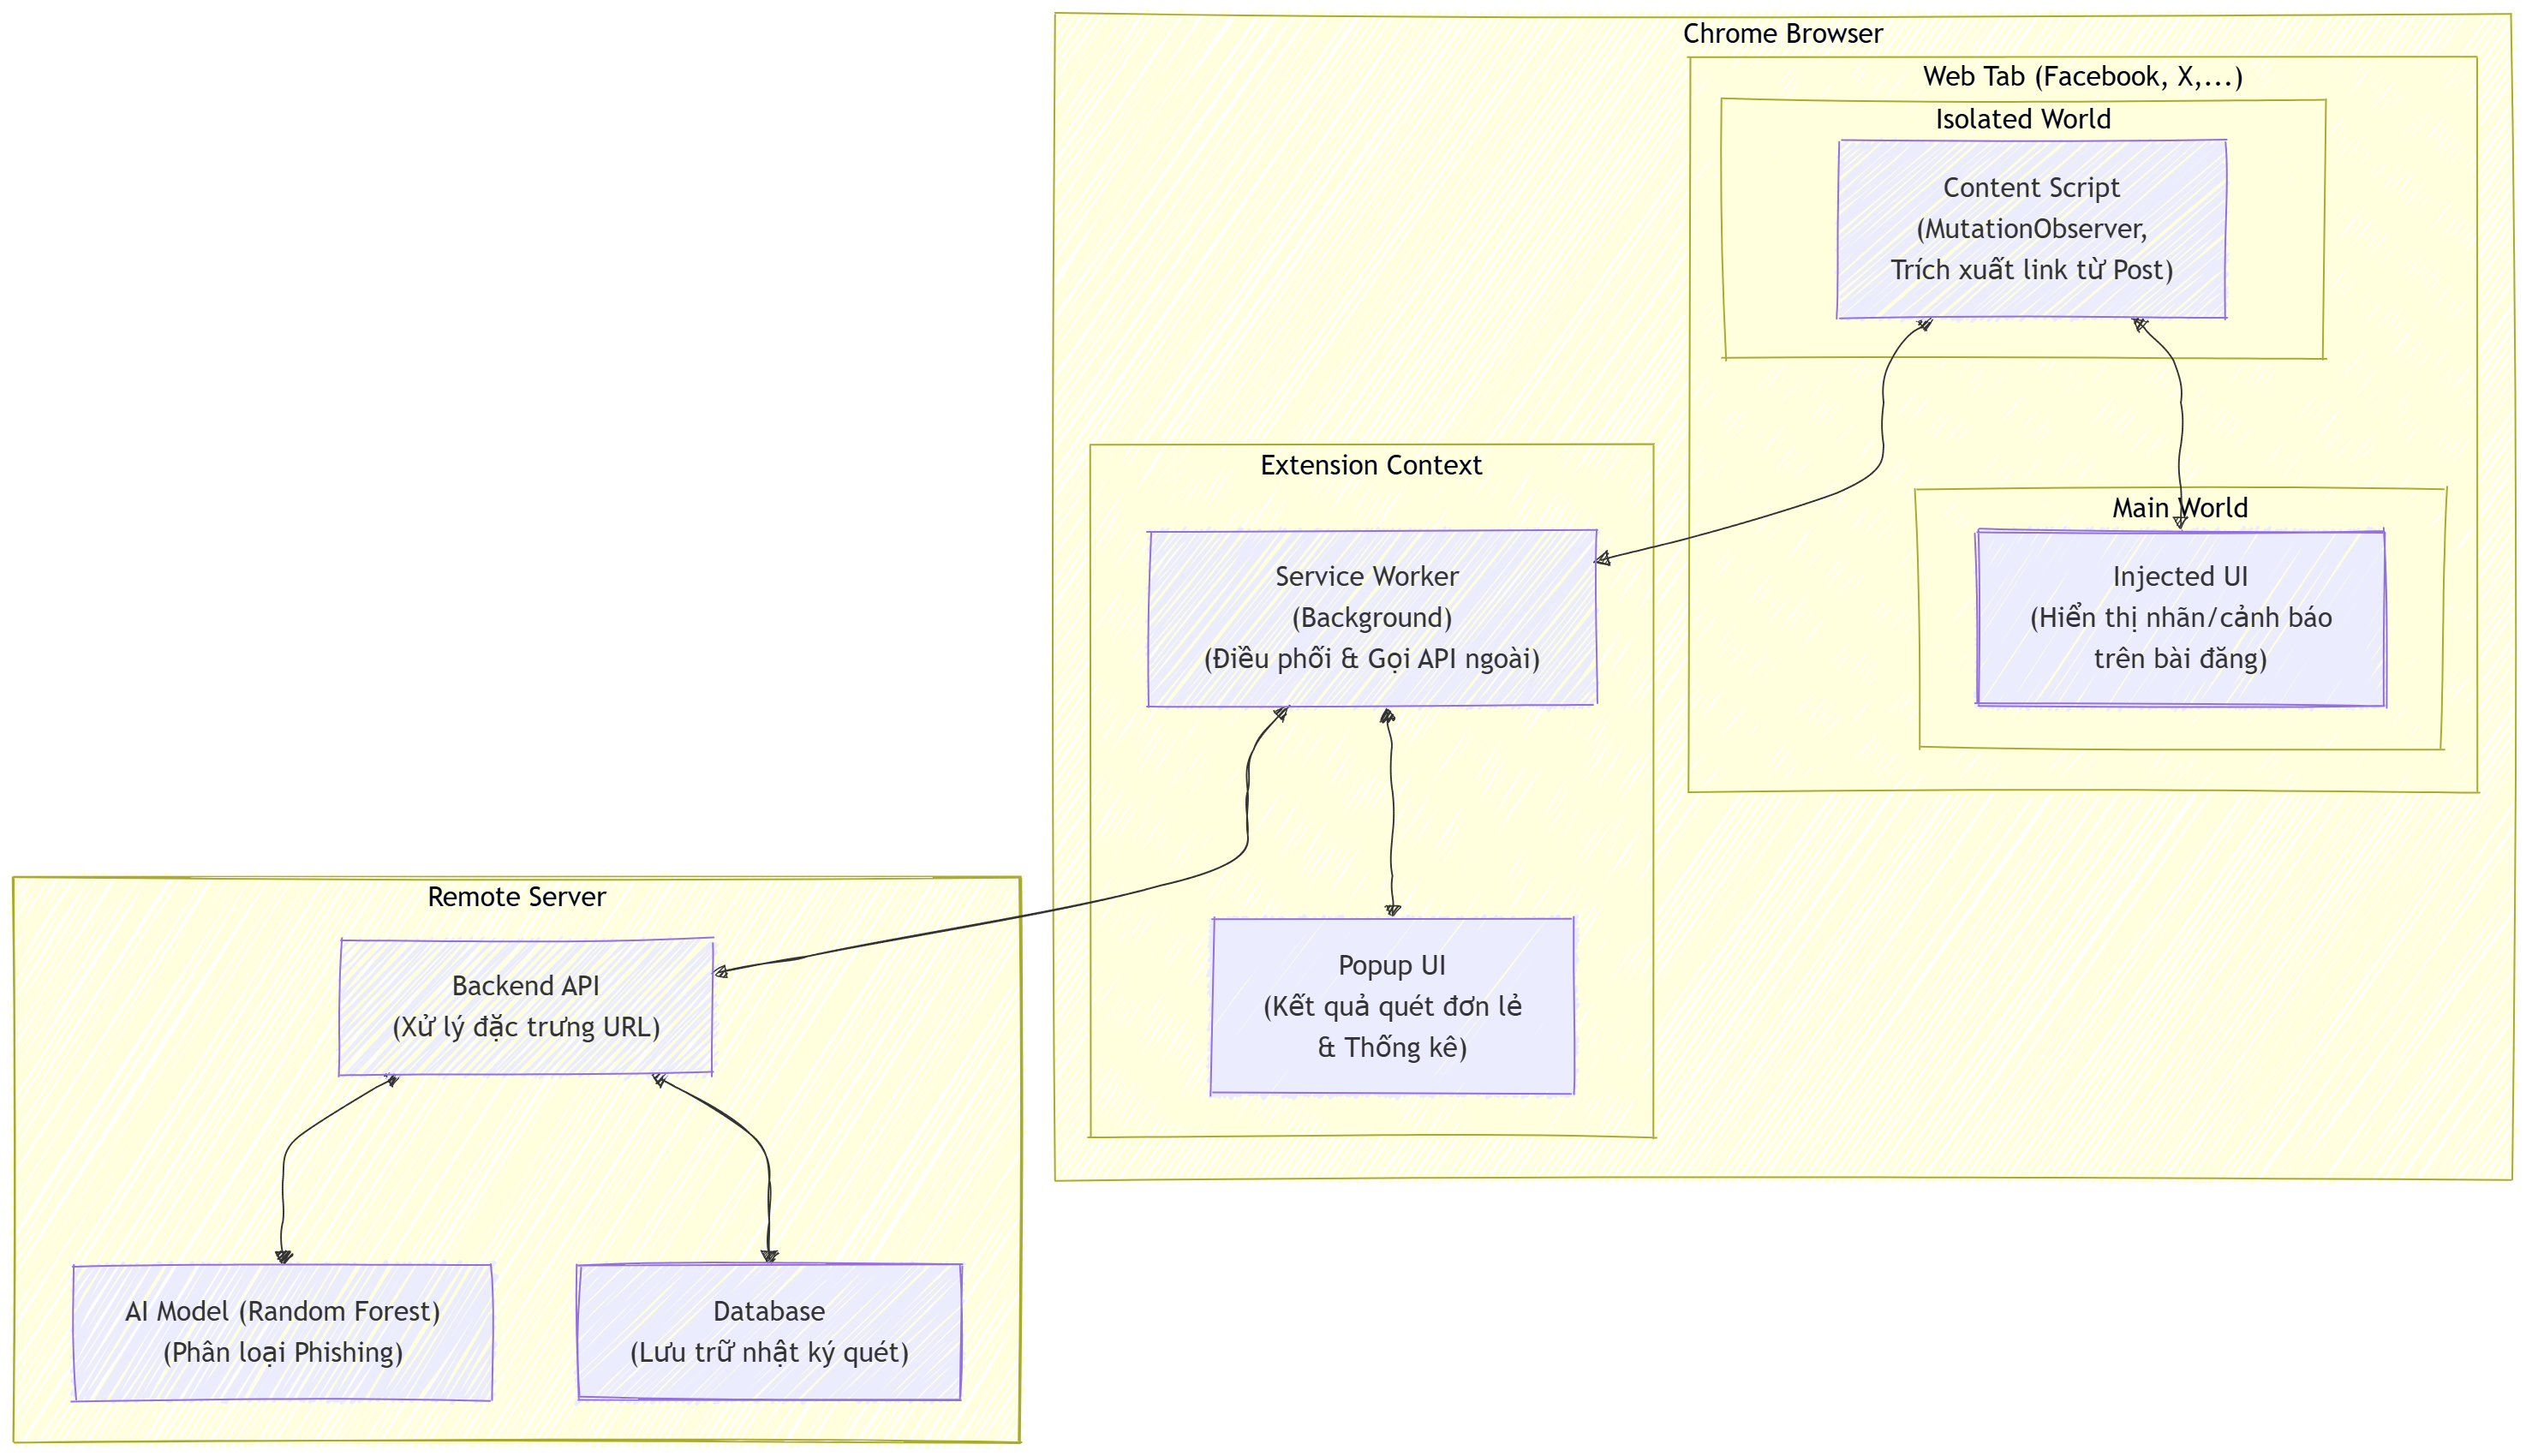
\includegraphics[width=0.9\textwidth]{figures/kien-truc -tien-ich.png} %
    \label{figures/kien-truc-extension}
\end{figure}

\subsection{Các thành phần chính của Extension (Client)}
Tiện ích được thiết kế tiêu chuẩn Manifest V3, kiến trúc phía Client được chia thành các khối thực thực thi nhiệm vụ riêng biệt và quyền hàng đặc trưng, các tương tác qua lại nhằm tối ưu hóa hiệu năng (Bên phải của hình \ref{figures/kien-truc-extension}).



\begin{itemize}
    \item Content Script (Tập lệnh nền): Chạy trong một ngữ cảnh biệt lập với JavaScript của trang web nhưng có quyền truy cập vào DOM. Thành phần này sử dụng API \texttt{MutationObserver} để giám sát các thay đổi động trên trang web (ví dụ: các bài đăng mới xuất hiện khi cuộn bảng tin). Nhiệm vụ chính là trích xuất các thẻ liên kết (\texttt{<a>}) và thực hiện thay đổi giao diện (UI Injection) để hiển thị cảnh báo.
    \item Background Script (Môi trường nền): Đây là bộ điều phối trung tâm của tiện ích. Nó lắng nghe các sự kiện từ Content Script, quản lý bộ nhớ đệm để giảm thiểu các yêu cầu lặp lại và thực hiện các giao tiếp HTTPS an toàn đến sever
    \item Popup UI: Giao diện hiển thị khi người dùng tương tác trực tiếp với biểu tượng tiện ích. Popup cung cấp các báo cáo chi tiết về mức độ tin cậy của đường dẫn trong bài viết.
\end{itemize}

\subsection{Kiến trúc hệ thống máy chủ (Remote Server)}
Phía máy chủ đảm nhận nhiệm vụ xử lý nặng, bao gồm việc bóc tách đặc trưng URL và vận hành mô hình dự đoán và lưu vào database những liên kết bị báo cáo(Bên trái của hình \ref{figures/kien-truc-extension}).

\begin{itemize}
    \item \textbf{Backend API:} Được xây dựng trên nền tảng FastAPI, đóng vai trò tiếp nhận URL từ Client và chuyển đổi chúng thành các vector đặc trưng số học (Feature Extraction) dựa trên các thuộc tính Lexical và DNS.
    \item \textbf{AI Model (Hybrid XGBoost):} Thành phần cốt lõi thực hiện phân loại nhị phân. Hệ thống sử dụng thuật toán XGBoost kết hợp với bộ lọc Heuristic (Khoảng cách Levenshtein) để đánh giá mức độ độc hại của liên kết.
    \item \textbf{Database:} Lưu trữ nhật ký quét (Scan logs) và danh sách đen (Blacklist) đã được xác nhận để tối ưu hóa tốc độ phản hồi cho các liên kết đã biết.
\end{itemize}

\section{Mô hình giao tiếp và luồng dữ liệu}
\label{sec:giao-tiep-he-thong}

Quy trình giao tiếp trong CheckPost được thiết kế đồng bộ để đảm bảo tính thời gian thực, thông qua cơ chế \textit{Chrome Message Passing}:

\begin{enumerate}
    \item \textbf{Giai đoạn Thu thập:} Content Script phát hiện liên kết mới trong bài đăng bài đăng qua \texttt{MutationObserver} và gửi URL về Service Worker thông qua hàm \texttt{chrome.runtime.sendMessage}.
    \item \textbf{Giai đoạn Gửi yêu cầu:} Background lắng nghe hàm chrome.runtime.onMessage kiểm tra URL trong bộ nhớ cục bộ. Nếu là URL mới, nó sẽ khởi tạo một yêu cầu HTTPS POST chứa dữ liệu URL đến Backend API tại Remote Server.
    \item \textbf{Giai đoạn Phân tích:} Backend thực hiện giải mã các link t.co, sau đó trích xuất 36 đặc trưng từ vựng và gửi vào bộ máy Hybrid (XGBoost + Heuristic) để lấy kết quả phân loại và các "cờ đỏ" (Red Flags) giải thích thông qua SHAP.
    \item \textbf{Giai đoạn Phản hồi:} Kết quả (Phishing/Legitimate) kèm theo độ tin cậy được trả về cho Service Worker. Cuối cùng, Service Worker phát tín hiệu để Content Script cập nhật nhãn cảnh báo ngay trên bài đăng người dùng đang xem và Popup để hiện thị các kết quả.
\end{enumerate}

\section{Thiết kế chức năng chi tiết}
\label{sec:thiet-ke-chuc-nang}

\subsection{Phân tích các liên kết trong bài đăng }
 Tiện ích sẽ phát hiện kết ngay khi chúng xuất hiện trên màn hình. Để giải quyết vấn đề của các trang web động (SPA), hệ thống không quét toàn bộ trang web một cách thụ động mà dựa trên các thay đổi cục bộ của cây DOM. Khi phát hiện đường dẫn mới  đợi 600 ms thì  thông qua hàm chrome.runtime.sendMessage Service Worker thì gửi lên cho server http Post để dự đoán mứa độ nguy hiểm của liên kết 
 
Hệ thống phân cấp mức độ nguy hiểm dựa trên điểm tin cậy từ mô hình AI minh họa hinh \ref{fig:kien-truc-server}:
\begin{enumerate}
    \item An toàn (Xanh):Tên miền có danh tiếng tốt, cấu trúc URL chuẩn.
    \item Cảnh báo (Vàng): URL chứa các yếu tố nghi vấn như có cấu trúc quá phức tạp và liên kết có nhiều dấu chấm.
    \item Nguy hiểm (Đỏ): Mô hình AI xác định là Phishing. Tiện ích sẽ kích hoạt lớp phủ bảo vệ ngăn người dùng nhấn vào liên kết.
\end{enumerate}
\begin{figure}[htbp]
    \centering 
    \caption{Giao diện pop-up hiện thị}
    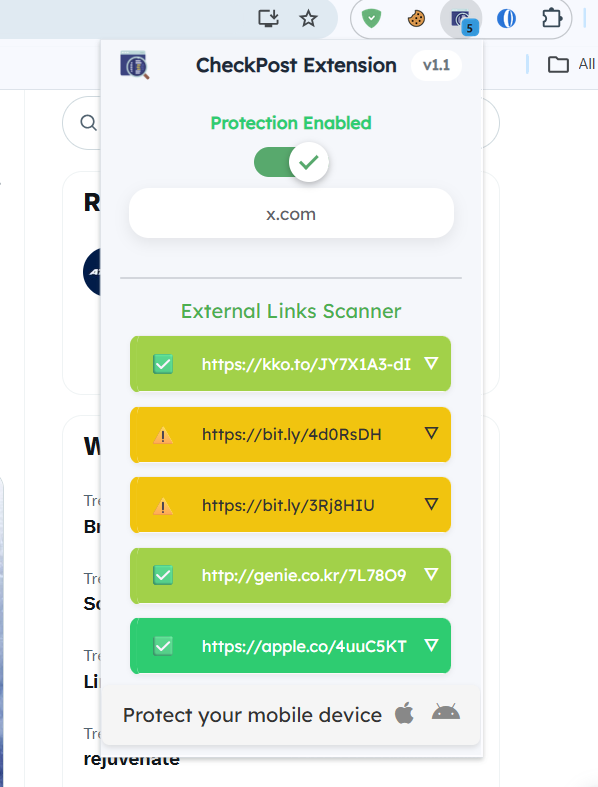
\includegraphics[width=0.8\textwidth]{figures/popup.png} 
    \label{fig:kien-truc-server}
\end{figure}
\subsection{Thách thức với liên kết rút gọn và cơ chế phân giải URL (\texttt{t.co})}

Khi đăng bài viết có chứa liên kết, X sẽ ngay lập tức thay thế URL gốc của bạn (ví dụ: https://yourdomain.com/long-article) bằng một liên kết t.co ngắn gọn và duy nhất (ví dụ: https://t.co/XYZ123). Quá trình này được gọi là đóng gói liên kết (link-wrapping).
Bản thân thao tác nhấp chuột sử dụng chuyển hướng HTTP 301 hoặc 302 tiêu chuẩn. Điều này có nghĩa là khi người dùng nhấp vào liên kết t.co, máy chủ của X sẽ ghi lại dữ liệu, thực hiện kiểm tra bảo mật, và sau đó ngay lập tức chuyển hướng người dùng đến URL đích ban đầu. Điều quan trọng là, URL đích ban đầu được che giấu khỏi người dùng nhưng được ghi lại và phân tích bởi hệ thống độc quyền của X cho mục đích theo dõi.
Trong môi trường mạng xã hội, đặc biệt là nền tảng X (Twitter), mọi liên kết ngoại vi đều được bọc qua dịch vụ rút gọn \texttt{t.co}. Điều này gây ra khó khăn lớn cho mô hình AI vì các đặc trưng Lexical (từ vựng) nguyên bản của trang web đích bị che giấu hoàn toàn dưới định dạng rút gọn (ví dụ: \texttt{https://t.co/xyz123}).

Để giải quyết vấn đề này, CheckPost triển khai cơ chế phân giải URL như sau:

Hệ thống được thiết kế để xử lý và mở rộng các liên kết rút gọn một cách nhanh chóng và hiệu quả, đặc biệt khi phải xử lý số lượng lớn URL cùng lúc. Đối với các liên kết như t.co của X, hệ thống không thể chỉ dựa vào cơ chế chuyển hướng HTTP thông thường (301/302) vì t.co thường trả về mã phản hồi 200 OK cùng một trang HTML chứa thẻ <meta refresh> để chuyển hướng. Do đó, hệ thống cần gửi yêu cầu GET để tải nội dung trang và sử dụng biểu thức chính quy (Regex) để trích xuất URL đích từ thẻ này. Cách làm này giúp vượt qua cơ chế chuyển hướng đặc biệt của t.co mà không cần sử dụng các công cụ nặng như trình duyệt tự động.

Để tối ưu hiệu năng, hệ thống sử dụng một AsyncClient duy nhất trong suốt vòng đời ứng dụng thay vì tạo mới kết nối cho mỗi yêu cầu. Điều này giúp tái sử dụng các kết nối mạng đã có (connection pooling), giảm thời gian thiết lập kết nối TCP/TLS và tăng tốc độ xử lý. Ngoài ra, trước khi gửi yêu cầu HTTP đến URL đích, hệ thống thực hiện kiểm tra DNS để xác minh tên miền có tồn tại hay không. Nếu tên miền không hợp lệ hoặc không thể phân giải, hệ thống sẽ dừng ngay thay vì phải chờ timeout từ yêu cầu HTTP, từ đó tiết kiệm tài nguyên và thời gian xử lý.

Bên cạnh đó, hệ thống còn sử dụng Semaphore để giới hạn số lượng yêu cầu được gửi đồng thời. Cơ chế này giúp tránh việc gửi quá nhiều request trong cùng một thời điểm, giảm nguy cơ bị máy chủ chặn hoặc gây quá tải tài nguyên mạng. Cuối cùng, mỗi URL sau khi xử lý đều được gắn trạng thái như resolved (xử lý thành công), dns_failed (lỗi DNS), hoặc unreachable (không thể kết nối máy chủ). Việc phân loại này giúp dễ dàng theo dõi lỗi, đánh giá chất lượng dữ liệu và hỗ trợ quá trình phân tích trong hệ thống phát hiện phishing

\subsection{Phân tích liên kết trong tin nhắn}
 Khi người dùng muốn kiểm tra mức độ an toàn của một đường dẫn liên kết, tiện ích mở rộng được thiết kế để hỗ trợ kiểm tra nhanh ngay trên giao diện trình duyệt mà không yêu cầu người dùng phải sao chép hoặc truy cập trực tiếp vào liên kết. Cụ thể, người dùng chỉ cần bôi đen (highlight) đoạn văn bản chứa liên kết cần kiểm tra trên trang web. Sau khi phát hiện người dùng đã chọn nội dung có chứa URL, hệ thống sẽ hiển thị một biểu tượng của tiện ích mở rộng ngay gần vị trí được chọn nhằm cung cấp thao tác kiểm tra trực quan và thuận tiện. Hình \ref{fig:giao dien scanning}
 \begin{figure}[htbp]
    \centering
    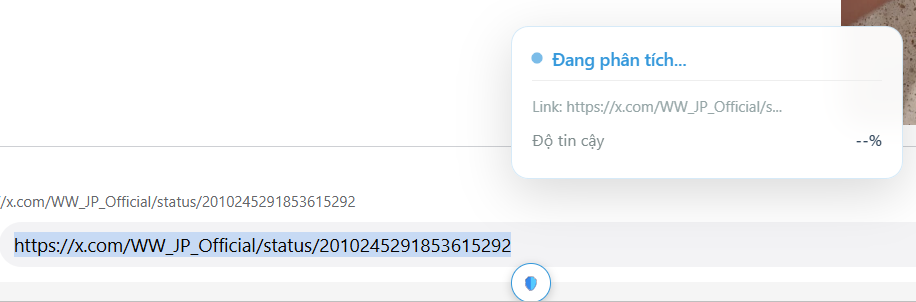
\includegraphics[width=0.8\textwidth]{figures/url_scanning.png} % Thay bằng tên file ảnh của bạn
    \caption{Giao diện pop-up hiện thị.}
    \label{fig:giao dien scanning}
\end{figure}

Khi người dùng nhấn vào biểu tượng này, content script được kích hoạt để tiến hành xử lý dữ liệu đầu vào. Ở bước này, content script sẽ thực hiện tiền xử lý liên kết bằng cách loại bỏ các ký tự không cần thiết hoặc nội dung nhiễu phát sinh trong quá trình người dùng bôi đen văn bản, chẳng hạn như dấu câu, ký tự đặc biệt hoặc khoảng trắng thừa. Đồng thời, hệ thống sử dụng biểu thức xử lý chuỗi để trích xuất chính xác phần nội dung bắt đầu từ giao thức mạng như http:// hoặc https:// cho đến trước ký tự khoảng trắng đầu tiên nhằm đảm bảo URL gửi đi có định dạng hợp lệ và giảm thiểu lỗi phân tích.

Sau khi hoàn tất bước tiền xử lý, content script gửi yêu cầu tới background script thông qua cơ chế truyền thông điệp nội bộ của tiện ích trình duyệt bằng lệnh:
chrome.runtime.sendMessage({action: "checkSingleLink",url: text})

Trong đó, thuộc tính action được sử dụng để xác định loại thao tác cần thực hiện, còn url chứa đường dẫn liên kết đã được làm sạch và chuẩn hóa. Background script đóng vai trò như một tầng trung gian chịu trách nhiệm giao tiếp với hệ thống backend. Sau khi nhận được thông điệp từ content script, background script sẽ gửi một HTTP POST request đến máy chủ phân tích nhằm kiểm tra mức độ an toàn của đường dẫn.

Tại phía server, liên kết được đưa vào quy trình phân tích gồm nhiều bước như mở rộng URL rút gọn (nếu có), trích xuất đặc trưng của tên miền và cấu trúc URL, kiểm tra các thuộc tính bảo mật, đồng thời đưa dữ liệu qua mô hình học máy để đánh giá nguy cơ lừa đảo (phishing). Sau khi hoàn tất quá trình suy luận, server trả về kết quả đánh giá bao gồm mức độ nguy hiểm, xác suất rủi ro hoặc nhãn phân loại của liên kết.

Khi nhận được dữ liệu phản hồi từ backend, content script tiếp tục xử lý phần giao diện người dùng bằng cách thao tác trực tiếp với DOM (Document Object Model) của trang web hiện tại. Hệ thống sẽ động tạo và chèn một thẻ HTML, chẳng hạn như phần tử <li>, vào vị trí phù hợp trên giao diện để hiển thị kết quả phân tích. Nội dung thông báo có thể bao gồm trạng thái như "Safe","Warning" và "Dangerous" đồng thời sử dụng màu sắc hoặc biểu tượng cảnh báo để giúp người dùng dễ dàng nhận biết mức độ rủi ro của trang web trước khi quyết định truy cập. Cách tiếp cận này giúp nâng cao trải nghiệm người dùng bằng việc cung cấp phản hồi gần như tức thời, trực quan và không làm gián đoạn quá trình duyệt web.


\section{Mô hình thuật toán AI và Trích xuất đặc trưng}
\label{sec:mo-hinh-ai-chi-tiet}

Hệ thống AI CheckPost áp dụng cơ chế \textbf{Hybrid Engine} (Động cơ lai) kết hợp giữa Học máy thống kê và Kiểm định kinh nghiệm:

\begin{enumerate}
    \item \textbf{Mô hình học máy XGBoost:} Sau quá trình làm sạch Data Leakage, mô hình XGBoost được tinh chỉnh với hàm mục tiêu Isotonic Regression. Nó xử lý xuất sắc các đặc trưng phi tuyến tính phức tạp của URL với tốc độ suy luận cực ngắn (dưới 1ms), đáp ứng yêu cầu phản hồi ngay lập tức.
    \item \textbf{Bộ lọc Typosquatting Heuristic:} Đối với các nhãn hiệu nổi tiếng (như Google, Facebook), mô hình tính toán khoảng cách Levenshtein giữa tên miền truy vấn và tên miền gốc. Nếu khoảng cách $\le 2$, nó tự động gắn cờ lừa đảo. Điều này bù đắp những thiếu sót của mô hình thống kê trước các cuộc tấn công nhắm mục tiêu (Spear-phishing).
    \item \textbf{Khả năng giải thích (Explainable AI):} Thay vì chỉ trả về "Có" hoặc "Không", mô hình tích hợp thuật toán \textbf{SHAP TreeExplainer} để trích xuất ra các \textit{Cờ đỏ (Red Flags)}—những lý do cụ thể khiến liên kết bị đánh giá nguy hiểm, từ đó cảnh báo trực quan cho người dùng.
\end{enumerate}

Dữ liệu đầu vào cho mô hình được bóc tách thành vector đặc trưng với 36 chiều $X$, bao gồm các thành phần quan trọng không rò rỉ dữ liệu như: độ dài tên miền, số lượng dấu chấm, sự hiện diện của địa chỉ IP, ký tự đặc biệt, và các hình thái từ vựng thống kê khác.

\subsection{Thiết kế cơ chế lưu trữ và Quản lý tri thức liên kết}
Để nâng cao hiệu suất và xây dựng cơ sở dữ liệu về các mối đe dọa, hệ thống triển khai mô hình lưu trữ phân cấp:

\begin{enumerate}
    \item \textbf{Lưu trữ cục bộ (Client-side Storage):}
    Sử dụng \texttt{chrome.storage.local} để lưu trữ các URL đã quét trong vòng 24 giờ. Dữ liệu được lưu dưới dạng bảng băm (Hash Map) với khóa là mã băm \texttt{SHA-256} của URL. Việc này giúp giảm kích thước lưu trữ và tăng tốc độ tìm kiếm khi người dùng quay lại các bài đăng cũ.
    
    \item \textbf{Cơ sở dữ liệu tập trung (Server-side Database):}
    Tại Remote Server, hệ thống sử dụng cơ sở dữ liệu để lưu trữ tri thức dài hạn bao gồm:
    \begin{itemize}
        \item \textbf{Bảng Blacklist:} Chứa các URL đã được mô hình AI xác nhận là phishing với độ tin cậy > 99\%.
        \item \textbf{Bảng Nhật ký (Audit Logs):} Lưu trữ lịch sử quét để thực hiện các báo cáo thống kê về xu hướng tấn công phishing theo thời gian.
    \end{itemize}
\end{enumerate}